\chapter{Camps magnètics d'espires i bobines}
\begin{resum}
	Aquesta pràctica té com a objectiu principal la mesura dels camps magnètics creats per diferents configuracions d'espires. Utilitzant un teslàmetre, s'han determinat experimentalment els camps creats, en el seu centre, per espires de radis diferents, així com per una, dues i tres espires concèntriques i amb el mateix radi i per diferents bobines en diversos punts del seu eix.

	Els resultats experimentals són consistents amb les prediccions teòriques, deduïdes a partir de la llei de Biot-Savart. En particular, s'ha observat la dependència del camp creat per una espira amb l'invers del seu radi o el fet que el camp creat per una bobina al seu eix és pràcticament constant a l'interior.
\end{resum}

\section{Introducció}
L'objectiu d'aquesta pràctica és mesurar i posteriorment analitzar els camps magnètics que resulten de la circulació de corrent elèctric per fils conductors. Més precisament, es disposarà de diverses espires i bobines per a la circulació del corrent. En el cas de les espires, es mesurarà el camp al centre d'espires de diferents radis i s'analitzarà la variació del camp en funció del radi. Per les bobines el que s'estudiarà és el camp magnètic a diferents punts de l'interior de bobines de diferent nombre de voltes i de diferents radis.

En relació al mencionat anteriorment, en aquest informe es presentaran gràfiques del camp magnètic al centre de l'espira en funció del radi d'aquesta i també del camp al centre en funció del nombre d'espires. Evidentment, també es proporcionarà el valor numèric dels diferents camps experimentals i teòrics, comparant els dos resultats i analitzant-ne la compatibilitat.

\section{Mètode experimental}
A continuació exposem els mètodes seguits per a l'obtenció de les dades experimentals en cada part de la pràctica.

\subsection{Espires}
Pel que fa a les espires, primerament s'ha muntat el circuit que inclou el teslàmetre amb la sonda, l'amperímetre, el regle i l'espira indicada en cada cas. La figura \cref{fig:esquema circuit} mostra un esquema d'aquest circuit.

\begin{figure}[htb]
  \centering
  % \includegraphics{Foto1.png}
  \caption{Esquema del circuit}
  \label{fig:esquema circuit}
\end{figure}

El propòsit del circuit de la figura \cref{fig:esquema circuit} és evidentment mesurar el camp al centre de l'espira. L'amperímetre ens resulta útil per obtenir una mesura més precisa que la donada pel generador de la intensitat que circula pel circuit. El teslàmetre indica el camp magnètic mesurat aproximadament a la punta de la sonda. Tanmateix, l'efectivitat del teslàmetre no és immediata i ha estat necessari esperar uns minuts perquè s'estabilitzi.

En concloure l'estabilització del teslàmetre, amb l'amperímetre marcant \SI{4.00}{A} , s'han pres mesures del camp col·locant la sonda al centre de l'espira. Concretament s'han pres 3 mesures en un sentit del corrent, tres mesures en l'altre i s'ha fet el promig per tal de compensar les fluctuacions del teslàmetre. Aquest procediment ha estat repetit per les tres espires a mesurar.

Posteriorment s'ha mesurat el camp al centre del conjunt de 1, 2 i 3 espires amb exactament el mateix procediment explicat.

El valor obtingut s'ha comparat amb l'esperat teòricament segons la fórmula obtinguda a partir de la llei de Biot i Savart:
\begin{equation}\label{eq:camp espira}
  \vec{B}=\frac{\mu_0 I N}{2 R}\hat{z}
\end{equation}
En la secció \cref{sec:espires} es presenten els resultats teòrics i experimentals d'aquest apartat, així com gràfics representant la variació del camp en funció del radi de l'espira i la variació en funció del nombre d'espires.

\subsection{Bobines}
Per la mesura del camp a l'interior de les bobines s'ha muntat el mateix circuit que s'ha il·lustrat a l'apartat anterior. 

Ajustant la intensitat a \SI{1.00}{A} a l'amperímetre, s'ha mesurat el camp a diversos punts a l'interior de la bobina. Per fer-ho s'ha ajustat l'alçada de la sonda de manera que aquesta quedi sobre l'eix interior de la bobina. Començant pel punt immediatament a l'exterior de la bobina s'ha fet avançar la sonda mesurant el camp cada \SI{3}{cm} (mesurats amb el regle) de manera que n'han resultat 8 mesures a diferents punts de l'eix.

Aquest mateix procediment s'ha repetit per cada bobina diferent i s'han comparat els valors amb els esperats de manera teòrica segons:
\begin{equation}
  \vec{B}=\frac{\mu_0 I N}{2 L}\left(\frac{z + L/2}{\sqrt{R^2+(z+L/2)^2}} - \frac{z - L/2}{\sqrt{R^2 + (z - L/2)^2}}\right)\hat{z}
\end{equation}

El valors teòrics i experimentals d'aquest apartat es presenten en la secció \cref{sec:bobines}.

\section{Presentació dels resultats}
En aquesta secció es presentaran i s'interpretaran els valors numèrics dels resultats obtinguts juntament amb algunes gràfiques representatives d'aquests resultats.

\subsection{Espires}\label{sec:espires}
Com s'ha mencionat anteriorment, en aquesta secció es presenten els resultats relatius a la part de la pràctica referent a les espires. Primerament es presenta la taula de la figura \cref{tab:espires} on apareixen els valors teòrics i experimentals del camp magnètic mesurat al centre de les tres espires de diferents radis.

\begin{figure}[htb]
  \centering
  % 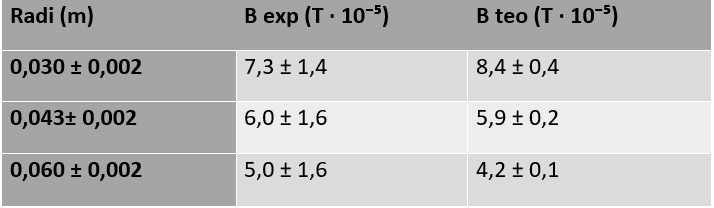
\includegraphics[width=100mm]{taul1.png}
  \caption{Taula de valors teòrics i experimentals}
  \label{tab:espires}
\end{figure}

Com podem veure en els tres casos, els valors experimentals amb els seus respectius intervals d'incertesa coincideixen en alguns punts amb els valors teòrics i els seus intervals, per tant els resultats són compatibles. Es pot observar que l'incertesa dels resultats experimentals és considerablement major. Això és degut a les imprecisions dels aparells emprats per a la mesura dels camps, especialment a les contínues fluctuacions del teslàmetre. 

Tanmateix, el fet més rellevant que podem observar és la disminució del camp a l'interior de l'espira a mesura que augmenta el seu radi. Aquest resultat ja era el que esperavem teòricament. Per fer més èmfasi en aquest fet es presenta la gràfica de la figura \cref{fig:camp espira}, on es representa el camp magnètic al centre en funció del radi de l'espira.
\begin{figure}[htb]
  \centering
  % 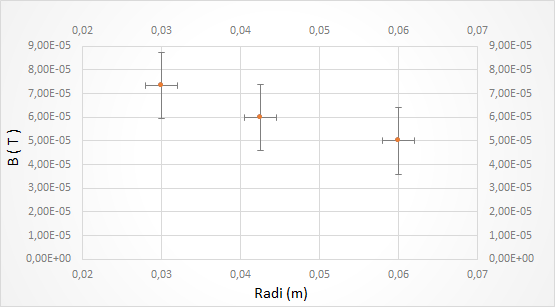
\includegraphics[width=100mm]{graf1.png}
  \caption{Camp magnètic al centre en funció del radi de l'espira}
  \label{fig:camp espira}
\end{figure}

Com es comentava, s'observa que el camp a l'interior es va  atenuant a mesura que s'augmenta el radi de l'espira. Tot i que és difícil d'apreciar ja que només s'ha fet la mesura amb tres radis diferents, es pot comprovar numèricament que el camp magnètic decau com \(\frac{1}{R}\). Aquesta és per tant la forma de funció que observaríem si es tinguessin valors infinits de radis d'espires i els seus camps respectius.

La taula de la figura \cref{fig:camp centre espires} presenta els camp magnètics teòrics i experimentals al centre dels conjunts de 1, 2 i 3 espires:

\begin{figure}[htb]
  \centering
  % 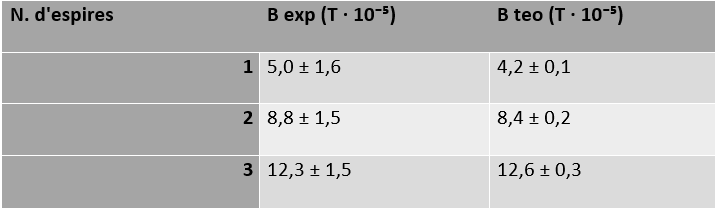
\includegraphics[width=100mm]{tau2a.png}
  \caption{Camps magnètics al centre dels conjunts d'espires}
  \label{fig:camp centre espires}
\end{figure}
Podem observar que en aquest cas els intervals dels camps teòrics i experimentals també se solapen i per tant les observacions satisfan l'esperat. Altra vegada tornem a tenir incerteses majors pels valors experimentals pel mateix fet anteriorment mencionat. Els resultats ens permeten observar que com més espires introduïm al conjunt més intens es torna el camp al centre d'aquest. Aquesta dependència es pot observar clarament al gràfic experimental del camp al centre en funció del nombre d'espires que s'exposa a la figura \cref{fig:camp vs n} :

\begin{figure}[htb]
  \centering
  % 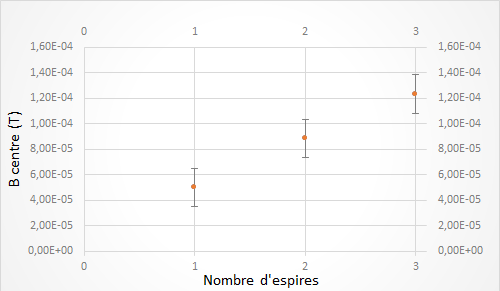
\includegraphics[width=100mm]{graf2.png}
  \caption{Camp al centre en funció del nombre d'espires}
  \label{fig:camp vs n}
\end{figure}

Podem veure al gràfic \cref{fig:camp vs n} que aquesta dependència és lineal com s'esperava dels valors teòrics obtinguts a partir de la fórmula \cref{eq:camp espira}. Així doncs, vist que el camp augmenta de manera directament proporcional al nombre d'espires, els resultats d'aquest apartat queden interpretats.

\subsection{Bobines}\label{sec:bobines}
Passant als resultats obtinguts per les bobines, comencem amb la bobina de 300 voltes i \SI{33}{mm} de diàmetre. A la taula de la figura \cref{fig:bobina 33 mm} es mostren els valors teòrics i els experimentals obtinguts juntament amb les seves incerteses del camp a diferents punts de l'interior a l'eix de la bobina:

\begin{figure}[htb]
  \centering
  % 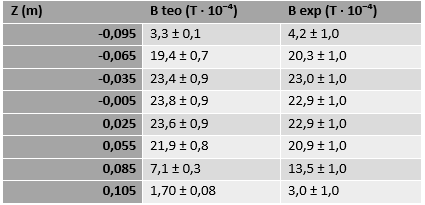
\includegraphics[width=100mm]{taubob1.png}
  \caption{Camp a punts de l'eix de la bobina de \SI{33}{mm}}
  \label{fig:bobina 33 mm}
\end{figure}

Podem observar que els diferents valors de camp coincideixen en la seva majoria. Tanmateix, en els punts més exteriors hi ha algunes incompatibilitats pel que fa als valors teòrics i experimentals. Aquestes diferències es deuen a la dificultat experimental per detectar l'acabament real de la bobina juntament amb el fet que teòricament el camp a l'exterior de la bobina decau molt ràpidament. No obstant, s'observa també el fet més rellevant: l'augment gradual del camp fins el punt més central on aquest és màxim i la posterior disminució del camp a mesura que els punts s'allunyen del centre. Aquest fet era el que s'esperava i el que indicaven els valors teòrics i s'ha pogut comprovar empíricament amb una precisió considerable.

Pel que fa a les bobines de \SI{26}{mm} de diàmetre, s'exposa a la figura \cref{tab:camp experimentals} una taula amb els valors empírics i a la figura \cref{tab:camps teorics} una altra amb els valors teòrics del camp a punts interiors de cadascuna.

\begin{figure}[htb]
  \centering
  % 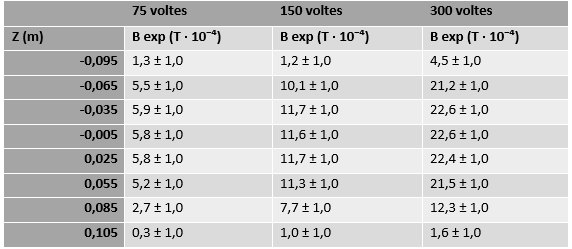
\includegraphics[width=100mm]{tau3exp.png}
  \caption{Valors experimentals del camp a les bobines}
  \label{tab:camp experimentals}
\end{figure}

\begin{figure}[htb]
  \centering
  % 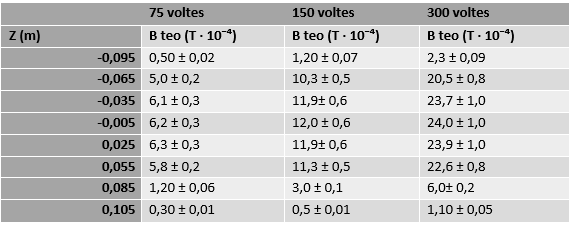
\includegraphics[width=100mm]{tau4teo.png}
  \caption{Valors teòrics del camp a les bobines}
  \label{tab:camps teorics}
\end{figure}

Els valors teòrics i els experimentals es comporten com en la bobina anterior. Tots els valors coincideixen en els seus intervals, exceptuant alguns valors a punts molt exteriors a la bobina que, pels efectes comentats anteriorment, presenten diferències. A part d'això, en aquest cas, a més d'observar correctament el mateix fet que en la bobina anterior, que el camp augmenta a l'entrar a la bobina i és màxim al centre, també observem l'efecte d'augmentar el nombre d'espires. Com esperàvem, el camp magnètic a l'interior de la bobina augmenta amb el nombre de voltes de la bobina. L'efecte teòric que s'esperava ha estat doncs confirmat per les observacions experimentals que indiquen aquest mateix fet.

\section{Conclusions}

En general els resultats obtinguts han estat satisfactoris. S'ha observat empíricament al llarg de tota la pràctica els fets que s'havien demostrat de manera teòrica. Els resultats més rellevants de la pràctica han estat els següents:
\begin{enumerate}
  \item El camp magnètic al centre d'una espira disminueix proporcionalment a \(\frac{1}{R}\) amb el radi.
  \item L'augment del nombre d'espires fa augmentar de manera lineal el camp al seu centre.
  \item El camp magnètic a l'eix d'una bobina és màxim en el seu centre.
  \item El camp magnètic d'una bobina augmenta amb el nombre de voltes d'aquesta.
\end{enumerate}
Es pot concloure per tant que la pràctica s'ha realitzat satisfactòriament.

\begin{figure}
	\sffamily \small
	\centering
	% GNUPLOT: LaTeX picture with Postscript
\begingroup
\sffamily \small
  \makeatletter
  \providecommand\color[2][]{%
    \GenericError{(gnuplot) \space\space\space\@spaces}{%
      Package color not loaded in conjunction with
      terminal option `colourtext'%
    }{See the gnuplot documentation for explanation.%
    }{Either use 'blacktext' in gnuplot or load the package
      color.sty in LaTeX.}%
    \renewcommand\color[2][]{}%
  }%
  \providecommand\includegraphics[2][]{%
    \GenericError{(gnuplot) \space\space\space\@spaces}{%
      Package graphicx or graphics not loaded%
    }{See the gnuplot documentation for explanation.%
    }{The gnuplot epslatex terminal needs graphicx.sty or graphics.sty.}%
    \renewcommand\includegraphics[2][]{}%
  }%
  \providecommand\rotatebox[2]{#2}%
  \@ifundefined{ifGPcolor}{%
    \newif\ifGPcolor
    \GPcolortrue
  }{}%
  \@ifundefined{ifGPblacktext}{%
    \newif\ifGPblacktext
    \GPblacktextfalse
  }{}%
  % define a \g@addto@macro without @ in the name:
  \let\gplgaddtomacro\g@addto@macro
  % define empty templates for all commands taking text:
  \gdef\gplbacktext{}%
  \gdef\gplfronttext{}%
  \makeatother
  \ifGPblacktext
    % no textcolor at all
    \def\colorrgb#1{}%
    \def\colorgray#1{}%
  \else
    % gray or color?
    \ifGPcolor
      \def\colorrgb#1{\color[rgb]{#1}}%
      \def\colorgray#1{\color[gray]{#1}}%
      \expandafter\def\csname LTw\endcsname{\color{white}}%
      \expandafter\def\csname LTb\endcsname{\color{black}}%
      \expandafter\def\csname LTa\endcsname{\color{black}}%
      \expandafter\def\csname LT0\endcsname{\color[rgb]{1,0,0}}%
      \expandafter\def\csname LT1\endcsname{\color[rgb]{0,1,0}}%
      \expandafter\def\csname LT2\endcsname{\color[rgb]{0,0,1}}%
      \expandafter\def\csname LT3\endcsname{\color[rgb]{1,0,1}}%
      \expandafter\def\csname LT4\endcsname{\color[rgb]{0,1,1}}%
      \expandafter\def\csname LT5\endcsname{\color[rgb]{1,1,0}}%
      \expandafter\def\csname LT6\endcsname{\color[rgb]{0,0,0}}%
      \expandafter\def\csname LT7\endcsname{\color[rgb]{1,0.3,0}}%
      \expandafter\def\csname LT8\endcsname{\color[rgb]{0.5,0.5,0.5}}%
    \else
      % gray
      \def\colorrgb#1{\color{black}}%
      \def\colorgray#1{\color[gray]{#1}}%
      \expandafter\def\csname LTw\endcsname{\color{white}}%
      \expandafter\def\csname LTb\endcsname{\color{black}}%
      \expandafter\def\csname LTa\endcsname{\color{black}}%
      \expandafter\def\csname LT0\endcsname{\color{black}}%
      \expandafter\def\csname LT1\endcsname{\color{black}}%
      \expandafter\def\csname LT2\endcsname{\color{black}}%
      \expandafter\def\csname LT3\endcsname{\color{black}}%
      \expandafter\def\csname LT4\endcsname{\color{black}}%
      \expandafter\def\csname LT5\endcsname{\color{black}}%
      \expandafter\def\csname LT6\endcsname{\color{black}}%
      \expandafter\def\csname LT7\endcsname{\color{black}}%
      \expandafter\def\csname LT8\endcsname{\color{black}}%
    \fi
  \fi
    \setlength{\unitlength}{0.0500bp}%
    \ifx\gptboxheight\undefined%
      \newlength{\gptboxheight}%
      \newlength{\gptboxwidth}%
      \newsavebox{\gptboxtext}%
    \fi%
    \setlength{\fboxrule}{0.5pt}%
    \setlength{\fboxsep}{1pt}%
\begin{picture}(5668.00,3400.00)%
    \gplgaddtomacro\gplbacktext{%
      \csname LTb\endcsname%%
      \put(946,704){\makebox(0,0)[r]{\strut{}\num{0}}}%
      \put(946,1117){\makebox(0,0)[r]{\strut{}\num{0.5}}}%
      \put(946,1529){\makebox(0,0)[r]{\strut{}\num{1}}}%
      \put(946,1942){\makebox(0,0)[r]{\strut{}\num{1.5}}}%
      \put(946,2354){\makebox(0,0)[r]{\strut{}\num{2}}}%
      \put(946,2767){\makebox(0,0)[r]{\strut{}\num{2.5}}}%
      \put(946,3179){\makebox(0,0)[r]{\strut{}\num{3}}}%
      \put(1078,484){\makebox(0,0){\strut{}\num{-15}}}%
      \put(1777,484){\makebox(0,0){\strut{}\num{-10}}}%
      \put(2476,484){\makebox(0,0){\strut{}\num{-5}}}%
      \put(3175,484){\makebox(0,0){\strut{}\num{0}}}%
      \put(3873,484){\makebox(0,0){\strut{}\num{5}}}%
      \put(4572,484){\makebox(0,0){\strut{}\num{10}}}%
      \put(5271,484){\makebox(0,0){\strut{}\num{15}}}%
    }%
    \gplgaddtomacro\gplfronttext{%
      \csname LTb\endcsname%%
      \put(198,1941){\rotatebox{-270}{\makebox(0,0){\strut{}$\mathsf{B \ (\si{mT})}$}}}%
      \put(3174,154){\makebox(0,0){\strut{}$\mathsf{z \ (\si{cm})}$}}%
    }%
    \gplbacktext
    \put(0,0){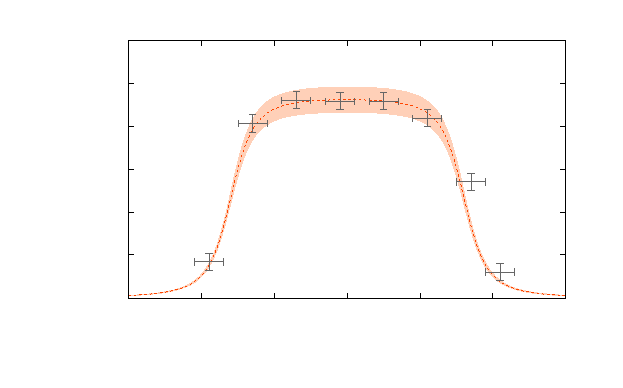
\includegraphics{camp-300-33}}%
    \gplfronttext
  \end{picture}%
\endgroup

	\caption{Camp magnètic al llarg de l'eix d'una espira de 300 voltes, longitud \SI{16}{cm} i diàmetre \SI{3.3}{cm} per la que hi passa un corrent constant de \SI{1}{A}.}
	\label{fig:camp 300/33}
\end{figure}

\begin{figure}
	\sffamily \small
	\centering
	% GNUPLOT: LaTeX picture with Postscript
\begingroup
\sffamily \small
  \makeatletter
  \providecommand\color[2][]{%
    \GenericError{(gnuplot) \space\space\space\@spaces}{%
      Package color not loaded in conjunction with
      terminal option `colourtext'%
    }{See the gnuplot documentation for explanation.%
    }{Either use 'blacktext' in gnuplot or load the package
      color.sty in LaTeX.}%
    \renewcommand\color[2][]{}%
  }%
  \providecommand\includegraphics[2][]{%
    \GenericError{(gnuplot) \space\space\space\@spaces}{%
      Package graphicx or graphics not loaded%
    }{See the gnuplot documentation for explanation.%
    }{The gnuplot epslatex terminal needs graphicx.sty or graphics.sty.}%
    \renewcommand\includegraphics[2][]{}%
  }%
  \providecommand\rotatebox[2]{#2}%
  \@ifundefined{ifGPcolor}{%
    \newif\ifGPcolor
    \GPcolortrue
  }{}%
  \@ifundefined{ifGPblacktext}{%
    \newif\ifGPblacktext
    \GPblacktextfalse
  }{}%
  % define a \g@addto@macro without @ in the name:
  \let\gplgaddtomacro\g@addto@macro
  % define empty templates for all commands taking text:
  \gdef\gplbacktext{}%
  \gdef\gplfronttext{}%
  \makeatother
  \ifGPblacktext
    % no textcolor at all
    \def\colorrgb#1{}%
    \def\colorgray#1{}%
  \else
    % gray or color?
    \ifGPcolor
      \def\colorrgb#1{\color[rgb]{#1}}%
      \def\colorgray#1{\color[gray]{#1}}%
      \expandafter\def\csname LTw\endcsname{\color{white}}%
      \expandafter\def\csname LTb\endcsname{\color{black}}%
      \expandafter\def\csname LTa\endcsname{\color{black}}%
      \expandafter\def\csname LT0\endcsname{\color[rgb]{1,0,0}}%
      \expandafter\def\csname LT1\endcsname{\color[rgb]{0,1,0}}%
      \expandafter\def\csname LT2\endcsname{\color[rgb]{0,0,1}}%
      \expandafter\def\csname LT3\endcsname{\color[rgb]{1,0,1}}%
      \expandafter\def\csname LT4\endcsname{\color[rgb]{0,1,1}}%
      \expandafter\def\csname LT5\endcsname{\color[rgb]{1,1,0}}%
      \expandafter\def\csname LT6\endcsname{\color[rgb]{0,0,0}}%
      \expandafter\def\csname LT7\endcsname{\color[rgb]{1,0.3,0}}%
      \expandafter\def\csname LT8\endcsname{\color[rgb]{0.5,0.5,0.5}}%
    \else
      % gray
      \def\colorrgb#1{\color{black}}%
      \def\colorgray#1{\color[gray]{#1}}%
      \expandafter\def\csname LTw\endcsname{\color{white}}%
      \expandafter\def\csname LTb\endcsname{\color{black}}%
      \expandafter\def\csname LTa\endcsname{\color{black}}%
      \expandafter\def\csname LT0\endcsname{\color{black}}%
      \expandafter\def\csname LT1\endcsname{\color{black}}%
      \expandafter\def\csname LT2\endcsname{\color{black}}%
      \expandafter\def\csname LT3\endcsname{\color{black}}%
      \expandafter\def\csname LT4\endcsname{\color{black}}%
      \expandafter\def\csname LT5\endcsname{\color{black}}%
      \expandafter\def\csname LT6\endcsname{\color{black}}%
      \expandafter\def\csname LT7\endcsname{\color{black}}%
      \expandafter\def\csname LT8\endcsname{\color{black}}%
    \fi
  \fi
    \setlength{\unitlength}{0.0500bp}%
    \ifx\gptboxheight\undefined%
      \newlength{\gptboxheight}%
      \newlength{\gptboxwidth}%
      \newsavebox{\gptboxtext}%
    \fi%
    \setlength{\fboxrule}{0.5pt}%
    \setlength{\fboxsep}{1pt}%
\begin{picture}(5668.00,3400.00)%
    \gplgaddtomacro\gplbacktext{%
      \csname LTb\endcsname%%
      \put(946,704){\makebox(0,0)[r]{\strut{}\num{0}}}%
      \put(946,1199){\makebox(0,0)[r]{\strut{}\num{0.2}}}%
      \put(946,1694){\makebox(0,0)[r]{\strut{}\num{0.4}}}%
      \put(946,2189){\makebox(0,0)[r]{\strut{}\num{0.6}}}%
      \put(946,2684){\makebox(0,0)[r]{\strut{}\num{0.8}}}%
      \put(946,3179){\makebox(0,0)[r]{\strut{}\num{1}}}%
      \put(1078,484){\makebox(0,0){\strut{}\num{-15}}}%
      \put(1777,484){\makebox(0,0){\strut{}\num{-10}}}%
      \put(2476,484){\makebox(0,0){\strut{}\num{-5}}}%
      \put(3175,484){\makebox(0,0){\strut{}\num{0}}}%
      \put(3873,484){\makebox(0,0){\strut{}\num{5}}}%
      \put(4572,484){\makebox(0,0){\strut{}\num{10}}}%
      \put(5271,484){\makebox(0,0){\strut{}\num{15}}}%
    }%
    \gplgaddtomacro\gplfronttext{%
      \csname LTb\endcsname%%
      \put(198,1941){\rotatebox{-270}{\makebox(0,0){\strut{}$\mathsf{B \ (\si{mT})}$}}}%
      \put(3174,154){\makebox(0,0){\strut{}$\mathsf{z \ (\si{cm})}$}}%
    }%
    \gplbacktext
    \put(0,0){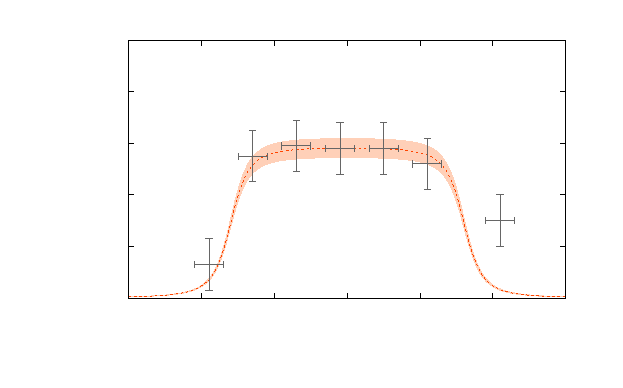
\includegraphics{camp-75-26}}%
    \gplfronttext
  \end{picture}%
\endgroup

	\caption{Camp magnètic al llarg de l'eix d'una espira de 75 voltes, longitud \SI{16}{cm} i diàmetre \SI{2.6}{cm} per la que hi passa un corrent constant de \SI{1}{A}.}
	\label{fig:camp 75/26}
\end{figure}

\begin{figure}
	\sffamily \small
	\centering
	% GNUPLOT: LaTeX picture with Postscript
\begingroup
\sffamily \small
  \makeatletter
  \providecommand\color[2][]{%
    \GenericError{(gnuplot) \space\space\space\@spaces}{%
      Package color not loaded in conjunction with
      terminal option `colourtext'%
    }{See the gnuplot documentation for explanation.%
    }{Either use 'blacktext' in gnuplot or load the package
      color.sty in LaTeX.}%
    \renewcommand\color[2][]{}%
  }%
  \providecommand\includegraphics[2][]{%
    \GenericError{(gnuplot) \space\space\space\@spaces}{%
      Package graphicx or graphics not loaded%
    }{See the gnuplot documentation for explanation.%
    }{The gnuplot epslatex terminal needs graphicx.sty or graphics.sty.}%
    \renewcommand\includegraphics[2][]{}%
  }%
  \providecommand\rotatebox[2]{#2}%
  \@ifundefined{ifGPcolor}{%
    \newif\ifGPcolor
    \GPcolortrue
  }{}%
  \@ifundefined{ifGPblacktext}{%
    \newif\ifGPblacktext
    \GPblacktextfalse
  }{}%
  % define a \g@addto@macro without @ in the name:
  \let\gplgaddtomacro\g@addto@macro
  % define empty templates for all commands taking text:
  \gdef\gplbacktext{}%
  \gdef\gplfronttext{}%
  \makeatother
  \ifGPblacktext
    % no textcolor at all
    \def\colorrgb#1{}%
    \def\colorgray#1{}%
  \else
    % gray or color?
    \ifGPcolor
      \def\colorrgb#1{\color[rgb]{#1}}%
      \def\colorgray#1{\color[gray]{#1}}%
      \expandafter\def\csname LTw\endcsname{\color{white}}%
      \expandafter\def\csname LTb\endcsname{\color{black}}%
      \expandafter\def\csname LTa\endcsname{\color{black}}%
      \expandafter\def\csname LT0\endcsname{\color[rgb]{1,0,0}}%
      \expandafter\def\csname LT1\endcsname{\color[rgb]{0,1,0}}%
      \expandafter\def\csname LT2\endcsname{\color[rgb]{0,0,1}}%
      \expandafter\def\csname LT3\endcsname{\color[rgb]{1,0,1}}%
      \expandafter\def\csname LT4\endcsname{\color[rgb]{0,1,1}}%
      \expandafter\def\csname LT5\endcsname{\color[rgb]{1,1,0}}%
      \expandafter\def\csname LT6\endcsname{\color[rgb]{0,0,0}}%
      \expandafter\def\csname LT7\endcsname{\color[rgb]{1,0.3,0}}%
      \expandafter\def\csname LT8\endcsname{\color[rgb]{0.5,0.5,0.5}}%
    \else
      % gray
      \def\colorrgb#1{\color{black}}%
      \def\colorgray#1{\color[gray]{#1}}%
      \expandafter\def\csname LTw\endcsname{\color{white}}%
      \expandafter\def\csname LTb\endcsname{\color{black}}%
      \expandafter\def\csname LTa\endcsname{\color{black}}%
      \expandafter\def\csname LT0\endcsname{\color{black}}%
      \expandafter\def\csname LT1\endcsname{\color{black}}%
      \expandafter\def\csname LT2\endcsname{\color{black}}%
      \expandafter\def\csname LT3\endcsname{\color{black}}%
      \expandafter\def\csname LT4\endcsname{\color{black}}%
      \expandafter\def\csname LT5\endcsname{\color{black}}%
      \expandafter\def\csname LT6\endcsname{\color{black}}%
      \expandafter\def\csname LT7\endcsname{\color{black}}%
      \expandafter\def\csname LT8\endcsname{\color{black}}%
    \fi
  \fi
    \setlength{\unitlength}{0.0500bp}%
    \ifx\gptboxheight\undefined%
      \newlength{\gptboxheight}%
      \newlength{\gptboxwidth}%
      \newsavebox{\gptboxtext}%
    \fi%
    \setlength{\fboxrule}{0.5pt}%
    \setlength{\fboxsep}{1pt}%
\begin{picture}(5668.00,3400.00)%
    \gplgaddtomacro\gplbacktext{%
      \csname LTb\endcsname%%
      \put(946,704){\makebox(0,0)[r]{\strut{}\num{0}}}%
      \put(946,1323){\makebox(0,0)[r]{\strut{}\num{0.5}}}%
      \put(946,1942){\makebox(0,0)[r]{\strut{}\num{1}}}%
      \put(946,2560){\makebox(0,0)[r]{\strut{}\num{1.5}}}%
      \put(946,3179){\makebox(0,0)[r]{\strut{}\num{2}}}%
      \put(1078,484){\makebox(0,0){\strut{}\num{-15}}}%
      \put(1777,484){\makebox(0,0){\strut{}\num{-10}}}%
      \put(2476,484){\makebox(0,0){\strut{}\num{-5}}}%
      \put(3175,484){\makebox(0,0){\strut{}\num{0}}}%
      \put(3873,484){\makebox(0,0){\strut{}\num{5}}}%
      \put(4572,484){\makebox(0,0){\strut{}\num{10}}}%
      \put(5271,484){\makebox(0,0){\strut{}\num{15}}}%
    }%
    \gplgaddtomacro\gplfronttext{%
      \csname LTb\endcsname%%
      \put(198,1941){\rotatebox{-270}{\makebox(0,0){\strut{}$\mathsf{B \ (\si{mT})}$}}}%
      \put(3174,154){\makebox(0,0){\strut{}$\mathsf{z \ (\si{cm})}$}}%
    }%
    \gplbacktext
    \put(0,0){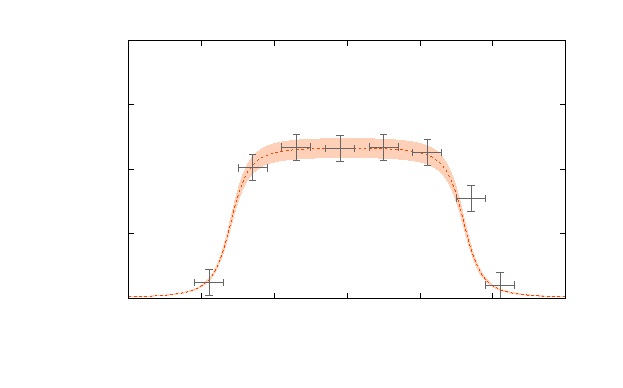
\includegraphics{camp-150-26}}%
    \gplfronttext
  \end{picture}%
\endgroup

	\caption{Camp magnètic al llarg de l'eix d'una espira de 150 voltes, longitud \SI{16}{cm} i diàmetre \SI{2.6}{cm} per la que hi passa un corrent constant de \SI{1}{A}.}
	\label{fig:camp 150/26}
\end{figure}

\begin{figure}
	\sffamily \small
	\centering
	% GNUPLOT: LaTeX picture with Postscript
\begingroup
\sffamily \small
  \makeatletter
  \providecommand\color[2][]{%
    \GenericError{(gnuplot) \space\space\space\@spaces}{%
      Package color not loaded in conjunction with
      terminal option `colourtext'%
    }{See the gnuplot documentation for explanation.%
    }{Either use 'blacktext' in gnuplot or load the package
      color.sty in LaTeX.}%
    \renewcommand\color[2][]{}%
  }%
  \providecommand\includegraphics[2][]{%
    \GenericError{(gnuplot) \space\space\space\@spaces}{%
      Package graphicx or graphics not loaded%
    }{See the gnuplot documentation for explanation.%
    }{The gnuplot epslatex terminal needs graphicx.sty or graphics.sty.}%
    \renewcommand\includegraphics[2][]{}%
  }%
  \providecommand\rotatebox[2]{#2}%
  \@ifundefined{ifGPcolor}{%
    \newif\ifGPcolor
    \GPcolortrue
  }{}%
  \@ifundefined{ifGPblacktext}{%
    \newif\ifGPblacktext
    \GPblacktextfalse
  }{}%
  % define a \g@addto@macro without @ in the name:
  \let\gplgaddtomacro\g@addto@macro
  % define empty templates for all commands taking text:
  \gdef\gplbacktext{}%
  \gdef\gplfronttext{}%
  \makeatother
  \ifGPblacktext
    % no textcolor at all
    \def\colorrgb#1{}%
    \def\colorgray#1{}%
  \else
    % gray or color?
    \ifGPcolor
      \def\colorrgb#1{\color[rgb]{#1}}%
      \def\colorgray#1{\color[gray]{#1}}%
      \expandafter\def\csname LTw\endcsname{\color{white}}%
      \expandafter\def\csname LTb\endcsname{\color{black}}%
      \expandafter\def\csname LTa\endcsname{\color{black}}%
      \expandafter\def\csname LT0\endcsname{\color[rgb]{1,0,0}}%
      \expandafter\def\csname LT1\endcsname{\color[rgb]{0,1,0}}%
      \expandafter\def\csname LT2\endcsname{\color[rgb]{0,0,1}}%
      \expandafter\def\csname LT3\endcsname{\color[rgb]{1,0,1}}%
      \expandafter\def\csname LT4\endcsname{\color[rgb]{0,1,1}}%
      \expandafter\def\csname LT5\endcsname{\color[rgb]{1,1,0}}%
      \expandafter\def\csname LT6\endcsname{\color[rgb]{0,0,0}}%
      \expandafter\def\csname LT7\endcsname{\color[rgb]{1,0.3,0}}%
      \expandafter\def\csname LT8\endcsname{\color[rgb]{0.5,0.5,0.5}}%
    \else
      % gray
      \def\colorrgb#1{\color{black}}%
      \def\colorgray#1{\color[gray]{#1}}%
      \expandafter\def\csname LTw\endcsname{\color{white}}%
      \expandafter\def\csname LTb\endcsname{\color{black}}%
      \expandafter\def\csname LTa\endcsname{\color{black}}%
      \expandafter\def\csname LT0\endcsname{\color{black}}%
      \expandafter\def\csname LT1\endcsname{\color{black}}%
      \expandafter\def\csname LT2\endcsname{\color{black}}%
      \expandafter\def\csname LT3\endcsname{\color{black}}%
      \expandafter\def\csname LT4\endcsname{\color{black}}%
      \expandafter\def\csname LT5\endcsname{\color{black}}%
      \expandafter\def\csname LT6\endcsname{\color{black}}%
      \expandafter\def\csname LT7\endcsname{\color{black}}%
      \expandafter\def\csname LT8\endcsname{\color{black}}%
    \fi
  \fi
    \setlength{\unitlength}{0.0500bp}%
    \ifx\gptboxheight\undefined%
      \newlength{\gptboxheight}%
      \newlength{\gptboxwidth}%
      \newsavebox{\gptboxtext}%
    \fi%
    \setlength{\fboxrule}{0.5pt}%
    \setlength{\fboxsep}{1pt}%
\begin{picture}(5668.00,3400.00)%
    \gplgaddtomacro\gplbacktext{%
      \csname LTb\endcsname%%
      \put(946,704){\makebox(0,0)[r]{\strut{}\num{0}}}%
      \put(946,1013){\makebox(0,0)[r]{\strut{}\num{0.5}}}%
      \put(946,1323){\makebox(0,0)[r]{\strut{}\num{1}}}%
      \put(946,1632){\makebox(0,0)[r]{\strut{}\num{1.5}}}%
      \put(946,1942){\makebox(0,0)[r]{\strut{}\num{2}}}%
      \put(946,2251){\makebox(0,0)[r]{\strut{}\num{2.5}}}%
      \put(946,2560){\makebox(0,0)[r]{\strut{}\num{3}}}%
      \put(946,2870){\makebox(0,0)[r]{\strut{}\num{3.5}}}%
      \put(946,3179){\makebox(0,0)[r]{\strut{}\num{4}}}%
      \put(1078,484){\makebox(0,0){\strut{}\num{-15}}}%
      \put(1777,484){\makebox(0,0){\strut{}\num{-10}}}%
      \put(2476,484){\makebox(0,0){\strut{}\num{-5}}}%
      \put(3175,484){\makebox(0,0){\strut{}\num{0}}}%
      \put(3873,484){\makebox(0,0){\strut{}\num{5}}}%
      \put(4572,484){\makebox(0,0){\strut{}\num{10}}}%
      \put(5271,484){\makebox(0,0){\strut{}\num{15}}}%
    }%
    \gplgaddtomacro\gplfronttext{%
      \csname LTb\endcsname%%
      \put(198,1941){\rotatebox{-270}{\makebox(0,0){\strut{}$\mathsf{B \ (\si{mT})}$}}}%
      \put(3174,154){\makebox(0,0){\strut{}$\mathsf{z \ (\si{cm})}$}}%
    }%
    \gplbacktext
    \put(0,0){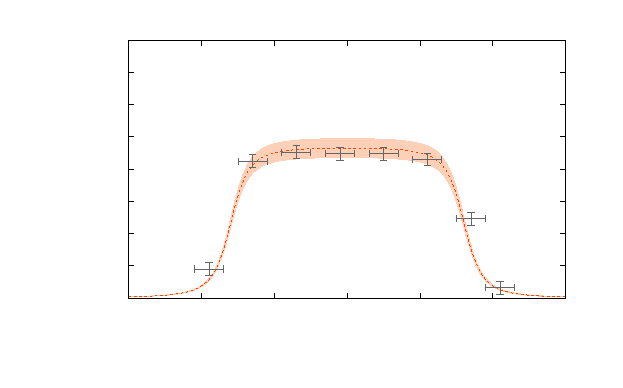
\includegraphics{camp-300-26}}%
    \gplfronttext
  \end{picture}%
\endgroup

	\caption{Camp magnètic al llarg de l'eix d'una espira de 300 voltes, longitud \SI{16}{cm} i diàmetre \SI{2.6}{cm} per la que hi passa un corrent constant de \SI{1}{A}.}
	\label{fig:camp 300/26}
\end{figure}
